\begin{enumerate}
	%
	\item 	
\begin{knitrout}
\definecolor{shadecolor}{rgb}{0.969, 0.969, 0.969}\color{fgcolor}\begin{kframe}
\begin{alltt}
\hlkwd{library}\hlstd{(ggplot2)}

\hlstd{f} \hlkwb{<-} \hlkwa{function}\hlstd{(}\hlkwc{x}\hlstd{,} \hlkwc{y}\hlstd{)} - \hlkwd{cos}\hlstd{(x}\hlopt{^}\hlnum{2} \hlopt{+} \hlstd{y}\hlopt{^}\hlnum{2} \hlopt{+} \hlstd{x}\hlopt{*}\hlstd{y)}
\hlstd{x} \hlkwb{=} \hlkwd{seq}\hlstd{(}\hlopt{-}\hlnum{2}\hlstd{,} \hlnum{2}\hlstd{,} \hlkwc{by}\hlstd{=}\hlnum{0.01}\hlstd{)}
\hlstd{xx} \hlkwb{=} \hlkwd{expand.grid}\hlstd{(}\hlkwc{X1} \hlstd{= x,} \hlkwc{X2} \hlstd{= x)}

\hlstd{fxx} \hlkwb{=} \hlkwd{f}\hlstd{(xx[, }\hlnum{1}\hlstd{], xx[, }\hlnum{2}\hlstd{])}
\hlstd{df} \hlkwb{=} \hlkwd{data.frame}\hlstd{(}\hlkwc{X1} \hlstd{= xx$X1,} \hlkwc{X2} \hlstd{= xx$X2,} \hlkwc{fxx} \hlstd{= fxx)}

\hlkwd{ggplot}\hlstd{(df,} \hlkwd{aes}\hlstd{(}\hlkwc{x} \hlstd{= X1,} \hlkwc{y} \hlstd{= X2,} \hlkwc{z} \hlstd{= fxx))} \hlopt{+}
  \hlkwd{geom_contour_filled}\hlstd{()} \hlopt{+}
  \hlkwd{xlab}\hlstd{(}\hlstr{"x1"}\hlstd{)} \hlopt{+}
  \hlkwd{ylab}\hlstd{(}\hlstr{"x2"}\hlstd{)}
\end{alltt}
\end{kframe}
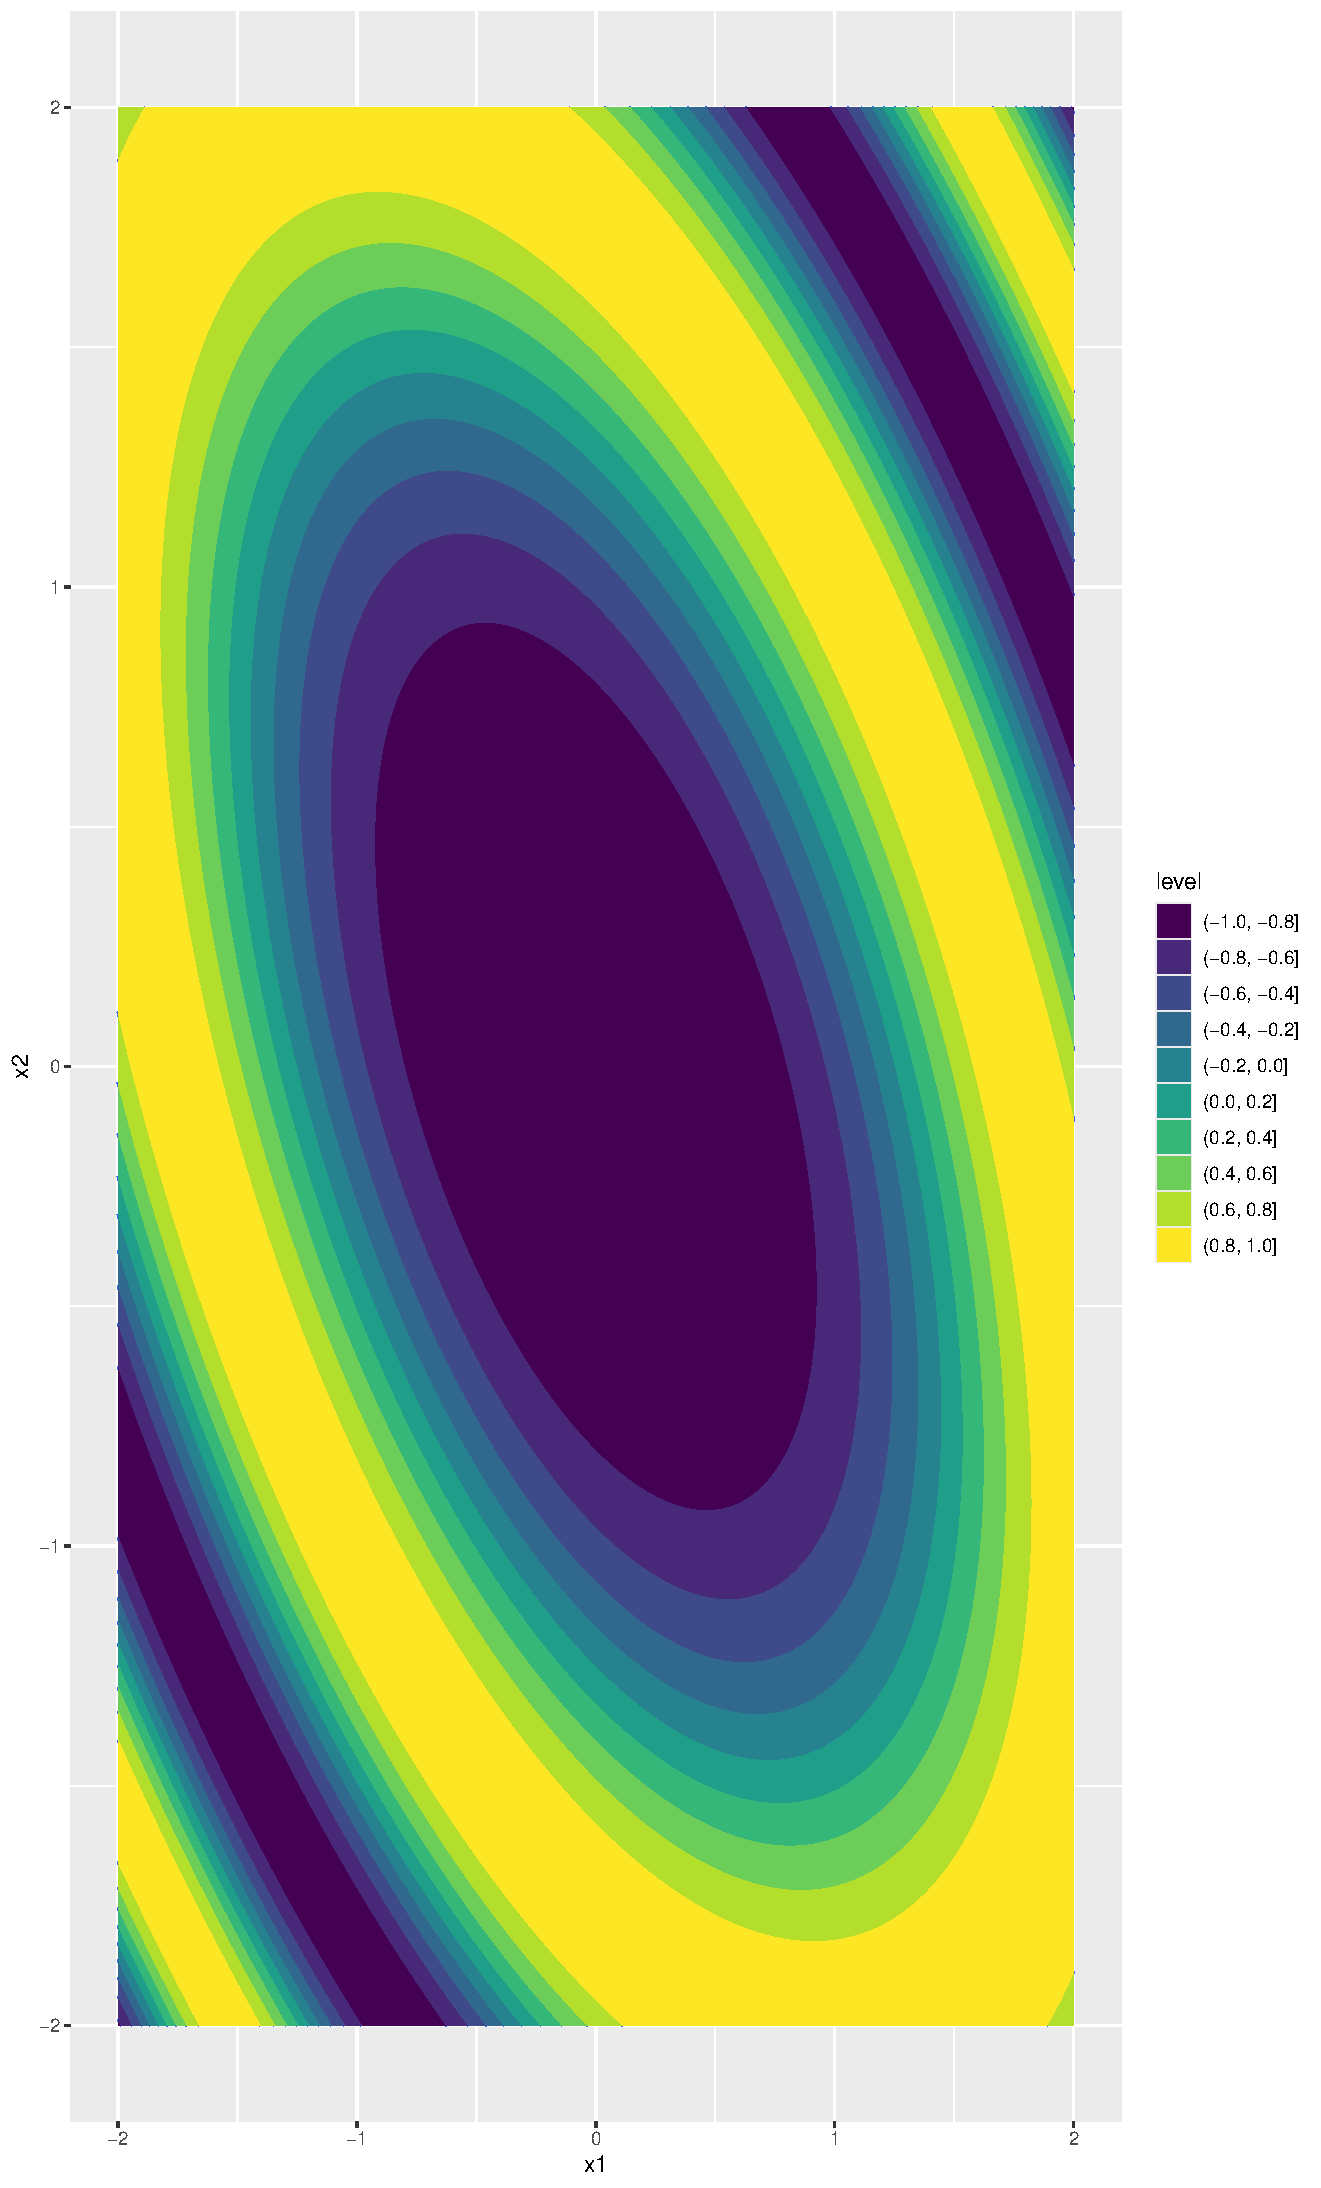
\includegraphics[width=0.5\linewidth]{figure/1d-plot-1} 
\end{knitrout}
\item $\nabla f = (\sin(x_1^2 + x_2^2 + x_1x_2)(2x_1 + x_2), \sin(x_1^2 + x_2^2 + x_1x_2)(2x_2 + x_1))^\top$
\item $\nabla^2 f = \begin{pmatrix} \cos(u)(2x_1 + x_2)^2 + 2\sin(u) & \cos(u)(2x_1 + x_2)(2x_2 + x_1) + \sin(u) \\ 
 \cos(u)(2x_1 + x_2)(2x_2 + x_1) + \sin(u) & \cos(u)(2x_2 + x_1)^2 + 2\sin(u)\end{pmatrix}$ with $u = x_1^2 + x_2^2 + x_1x_2.$
 \item Let $\mathbf{u}: \R^2 \rightarrow \R, (x_1, x_2) \mapsto x_1^2 + x_2^2 + x_1x_2$. \\ % and $g:\R \rightarrow \R, u \mapsto -\cos(u)$. 
 $\nabla^2 \mathbf{u} = \begin{pmatrix} 2 & 1 \\ 1 & 2\end{pmatrix} \Rightarrow \mathbf{v}^\top \nabla^2 \mathbf{u} \mathbf{v} = 2 v_1^2 + 2v_1v_2 + 2 v_2^2 = v_1^2 + v_2^2 + (v_1 + v_2)^2 \geq 0$ (equality only holds if $\mathbf{v} = \mathbf{0}$) $\Rightarrow \nabla^2 \mathbf{u}$ is positive definite. \\
 $    \frac{\partial^2}{\partial \mathbf{x} \partial \mathbf{x}^\top}-\cos(\mathbf{u}(\mathbf{x})) =$
	
\end{enumerate}
